% TikZ Diagram: S2 Linear Recurrent Unit (S2-LRU) context bank
% Style: Minimal publication palette (Grayscale structural + Single Accent for proposed module)
% Rules: Rectangles = Operations/Modules, Rounded = Data/Tensors. Left-to-right flow. Zero line crossing.

\documentclass[tikz,border=10pt]{standalone}
\usetikzlibrary{shapes.geometric, positioning, arrows.meta, chains, backgrounds}

\definecolor{neutralbg}{HTML}{F8FAFC}
\definecolor{neutralstroke}{HTML}{64748B}
\definecolor{neutraltext}{HTML}{0F172A}

\definecolor{accentbg}{HTML}{FEF3C7}
\definecolor{accentstroke}{HTML}{D97706}
\definecolor{accenttext}{HTML}{92400E}

\begin{document}
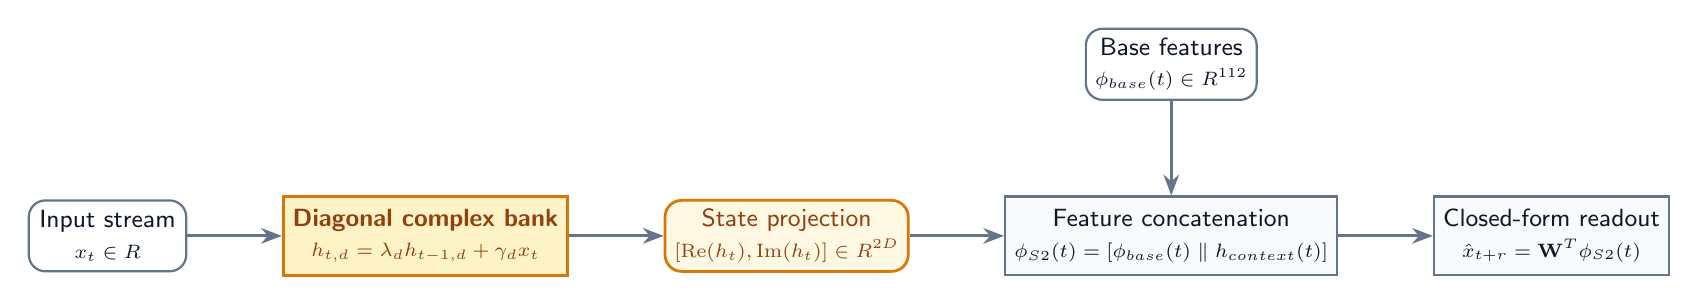
\begin{tikzpicture}[
    font=\sffamily\small,
    node distance=1.0cm and 1.2cm,
    operation/.style={rectangle, draw=neutralstroke, fill=neutralbg, text=neutraltext, minimum height=1.0cm, minimum width=2.2cm, align=center, line width=0.8pt},
    proposed_op/.style={rectangle, draw=accentstroke, fill=accentbg, text=accenttext, minimum height=1.0cm, minimum width=2.4cm, align=center, line width=1.2pt, font=\sffamily\bfseries\small},
    tensor/.style={rounded corners=6pt, draw=neutralstroke, fill=white, text=neutraltext, minimum height=0.9cm, minimum width=2.0cm, align=center, line width=0.8pt},
    proposed_tensor/.style={rounded corners=6pt, draw=accentstroke, fill=accentbg!50, text=accenttext, minimum height=0.9cm, minimum width=2.2cm, align=center, line width=1.0pt},
    arrow/.style={-{Stealth[scale=1.0]}, line width=1.0pt, draw=neutralstroke},
    aux_arrow/.style={-{Stealth[scale=1.0]}, line width=1.0pt, draw=accentstroke, dashed}
]

    % Input stream
    \node[tensor] (input) {Input stream\\{\scriptsize $x_t \in \mathbb{R}$}};

    % Proposed S2-LRU recurrent bank
    \node[proposed_op, right=of input] (lru) {Diagonal complex bank\\{\scriptsize $h_{t,d} = \lambda_d h_{t-1,d} + \gamma_d x_t$}};

    % State projection
    \node[proposed_tensor, right=of lru] (context) {State projection\\{\scriptsize $[\mathrm{Re}(h_t), \mathrm{Im}(h_t)] \in \mathbb{R}^{2D}$}};

    % Concatenation
    \node[operation, right=of context] (concat) {Feature concatenation\\{\scriptsize $\phi_{\text{S2}}(t) = [\phi_{\text{base}}(t) \parallel h_{\text{context}}(t)]$}};

    % Closed-form readout
    \node[operation, right=of concat] (readout) {Closed-form readout\\{\scriptsize $\hat{x}_{t+r} = \mathbf{W}^T \phi_{\text{S2}}(t)$}};

    % Base feature input
    \node[tensor, above=1.2cm of concat] (base) {Base features\\{\scriptsize $\phi_{\text{base}}(t) \in \mathbb{R}^{112}$}};

    % Flow arrows
    \draw[arrow] (input) -- (lru);
    \draw[arrow] (lru) -- (context);
    \draw[arrow] (context) -- (concat);
    \draw[arrow] (base) -- (concat);
    \draw[arrow] (concat) -- (readout);

\end{tikzpicture}
\end{document}
